\documentclass[conference]{IEEEtran}
%% SECON 2013 addition:
\makeatletter
\def\ps@headings{%
\def\@oddhead{\mbox{}\scriptsize\rightmark \hfil \thepage}%
\def\@evenhead{\scriptsize\thepage \hfil \leftmark\mbox{}}%
\def\@oddfoot{}%
\def\@evenfoot{}}
\makeatother
\pagestyle{headings} 

\ifCLASSINFOpdf
  % \usepackage[pdftex]{graphicx}
  % declare the path(s) where your graphic files are
  % \graphicspath{{../pdf/}{../jpeg/}}
  % and their extensions so you won't have to specify these with
  % every instance of \includegraphics
  % \DeclareGraphicsExtensions{.pdf,.jpeg,.png}
\else
  % or other class option (dvipsone, dvipdf, if not using dvips). graphicx
  % will default to the driver specified in the system graphics.cfg if no
  % driver is specified.
  % \usepackage[dvips]{graphicx}
  % declare the path(s) where your graphic files are
  % \graphicspath{{../eps/}}
  % and their extensions so you won't have to specify these with
  % every instance of \includegraphics
  % \DeclareGraphicsExtensions{.eps}
\fi
% *** MATH PACKAGES ***
%
\usepackage[cmex10]{amsmath}
\usepackage{amsfonts}
\usepackage{graphicx, epsfig}
\usepackage{color}
\usepackage{subfigure}
\usepackage{xspace}
\usepackage{algorithm}
\usepackage{algpseudocode}
\usepackage{breqn}
\usepackage{cite}

\renewcommand{\thealgorithm}{}
\algnewcommand{\LineComment}[1]{\State \(\triangleright\) #1}
% A popular package from the American Mathematical Society that provides
% many useful and powerful commands for dealing with mathematics. If using
% it, be sure to load this package with the cmex10 option to ensure that
% only type 1 fonts will utilized at all point sizes. Without this option,
% it is possible that some math symbols, particularly those within
% footnotes, will be rendered in bitmap form which will result in a
% document that can not be IEEE Xplore compliant!
%
%\usepackage{array}
%\usepackage{mdwmath}
%\usepackage{mdwtab}
%\usepackage{eqparbox}
%\usepackage[tight,footnotesize]{subfigure}
%\usepackage[caption=false]{caption}
%\usepackage[font=footnotesize]{subfig}
%\usepackage[caption=false,font=footnotesize]{subfig}
%
%\usepackage{fixltx2e}

%\usepackage{stfloats}

%\usepackage{url}

% correct bad hyphenation here
\hyphenation{net-works}

\DeclareMathOperator*{\E}{\mathbb{E}}

\begin{document}
%
% paper title
% can use linebreaks \\ within to get better formatting as desired
\title{QoI Symptotics - Timeliness Example}

\IEEEoverridecommandlockouts

% author names and affiliations
% use a multiple column layout for up to three different
% affiliations

%\author{\IEEEauthorblockN{Scott Rager}
%\IEEEauthorblockA{Department of Computer Science and Engineering\\
%Pennsylvania State University\\
%University Park, PA 16802\\
%Email: rager@psu.edu}}

%\author{\IEEEauthorblockN{Scott Rager, Ertugrul Ciftcioglu, Thomas La Porta}
%\IEEEauthorblockA{Department of Computer Science\\
%and Engineering\\
%Pennsylvania State University\\
%University Park, PA 16802\\
%Email: rager@psu.edu, enc118@psu.edu, tlp@cse.psu.edu}
%\and
%\IEEEauthorblockN{Alice Leung, William Dron}
%\IEEEauthorblockA{Raytheon BBN Technologies\\
%Cambridge, MA 02138\\
%Email: aleung@bbn.com, wdron@bbn.com}
%\and
%\IEEEauthorblockN{John Hancock}
%\IEEEauthorblockA{Artistech\\
%City, State Zip Code\\
%Email: johnh@artistech.com}
%}

%\author{
%  \IEEEauthorblockN{Scott T. Rager\IEEEauthorrefmark{1} \quad Ertugrul N. Ciftcioglu\IEEEauthorrefmark{1} \quad
%    \quad Thomas F. La Porta\IEEEauthorrefmark{1} \\ Alice Leung\IEEEauthorrefmark{2} \quad William Dron\IEEEauthorrefmark{2} \quad John Hancock\IEEEauthorrefmark{3} \\
%  }
%  \IEEEauthorblockA{
%  	\IEEEauthorrefmark{1}The Pennsylvania State University, University Park, PA 16802\\
%  \IEEEauthorrefmark{2}Raytheon BBN Technologies, Cambridge, MA 02138\\
%  \IEEEauthorrefmark{3}Artistech, Inc., Fairfax, VA 22030
%  }
%
%  Email:  str5004@psu.edu, enc118@psu.edu, tlp@cse.psu.edu, aleung@bbn.com, wdron@bbn.com, johnh@artistech.com
%\thanks{Research was sponsored by the U.S. Army Research Laboratory under the Network Science Collaborative Technology Alliance, Agreement Number W911NF-09-2-0053.} }


% for over three affiliations, or if they all won't fit within the width
% of the page, use this alternative format:
% 
%\author{\IEEEauthorblockN{Michael Shell\IEEEauthorrefmark{1},
%Homer Simpson\IEEEauthorrefmark{2},
%James Kirk\IEEEauthorrefmark{3}, 
%Montgomery Scott\IEEEauthorrefmark{3} and
%Eldon Tyrell\IEEEauthorrefmark{4}}
%\IEEEauthorblockA{\IEEEauthorrefmark{1}School of Electrical and Computer Engineering\\
%Georgia Institute of Technology,
%Atlanta, Georgia 30332--0250\\ Email: see http://www.michaelshell.org/contact.html}
%\IEEEauthorblockA{\IEEEauthorrefmark{2}Twentieth Century Fox, Springfield, USA\\
%Email: homer@thesimpsons.com}
%\IEEEauthorblockA{\IEEEauthorrefmark{3}Starfleet Academy, San Francisco, California 96678-2391\\
%Telephone: (800) 555--1212, Fax: (888) 555--1212}
%\IEEEauthorblockA{\IEEEauthorrefmark{4}Tyrell Inc., 123 Replicant Street, Los Angeles, California 90210--4321}}




% use for special paper notices
%\IEEEspecialpapernotice{(Invited Paper)}




% make the title area
\maketitle


\begin{abstract}
\boldmath
Explanation using delay instead of bandwidth:
%%area
%Practical network scalability, known as \emph{symptotics}, has obvious applications in designing ad hoc networks.  
%%problem
%In any practical implementation, knowing the limitations on scalability, the capabilities of deliverable QoI, and the impact of QoI requirements are crucial to designing an operational, effective network.
%%solution
%To obtain upper limits on network scalability and, more importantly, to understand how these limits are impacted by QoI functions and requirements, we apply QoI awareness to the symptotics framework.
%%methodology
%We use two similarity-based image retrieval algorithms to motivate and exemplify the relationship between timely QoI requirements and network scalability.
%%results
%Results show that high QoI and strict timeliness requirements can have a large impact on scalability, which gives a much clearer understanding of the tradeoffs present in network design.  We also introduce and show examples of \emph{scalably feasible QoI regions} for special cases, showing clear limitations on QoI requirements that are able to be satisfied by these networks.
%%takeaway

\end{abstract}

% IEEEtran.cls defaults to using nonbold math in the Abstract.
% This preserves the distinction between vectors and scalars. However,
% if the conference you are submitting to favors bold math in the abstract,
% then you can use LaTeX's standard command \boldmath at the very start
% of the abstract to achieve this. Many IEEE journals/conferences frown on
% math in the abstract anyway.

% no keywords




% For peer review papers, you can put extra information on the cover
% page as needed:
% \ifCLASSOPTIONpeerreview
% \begin{center} \bfseries EDICS Category: 3-BBND \end{center}
% \fi
%
% For peerreview papers, this IEEEtran command inserts a page break and
% creates the second title. It will be ignored for other modes.
\IEEEpeerreviewmaketitle

%\begin{abstract}
%
%In many deployments of mobile ad hoc networks (MANETs), the primary goal is to collect and deliver data from many nodes to a designated operation center to support situation awareness and decision-making.  Additionally, this goal must be met while considering the limited resources, such as battery life, in the wireless nodes.  Traditional MANET protocols and research focus on providing protocols that are evaluated on performance criteria such as throughput and delay.  In this work, we extend this notion to include emphasis on the usefulness of data content along with traditional network state indicators such as current channel conditions to make cross-layer control decisions.  First we develop the notion of an information space created by generated data. Next, we formulate the problem of maximizing coverage over this information space while restricting individual node costs to remain within a given budget.  We then provide an algorithm that provides the solution to this problem.  Next we consider the related problem of finding the optimal long-term average coverage subject to average cost constraints and give its solution, which uses Lyapunov Optimization techniques.  For real world implementations, we also provide computationally feasible approximation algorithms for optimal solutions of both problems, including a novel technique that uses virtual queues for the average maximum coverage problem.  Finally, we provide simulation results of all proposed algorithms.  These results not only demonstrate the benefits of considering data content in scheduling, but also show the advantages from using the long-term average solution and the near-optimal performance of our greedy virtual queue approximation algorithm.
%
%\end{abstract}

\section{Explanation}

Instead of looking at bandwidth, which we have been doing and which is the basis for the previous symptotics work, flipping the problem a bit might provide a more intuitive look, but we'll see that the result is the same.  We look at a single flow that must complete in a timeliness of $T$ seconds.  We will say that the flow has a QoI requirement that results in the need for $B$ bits, fragmented into packets of size $P$ bits, to be sent from each source to each destination.  The rate of each link is $W$ bits per second.

Now, we have two contributors to delay.  The first contributor is the end to end delay incurred by sending the $B$ bits across the entire path.  Here, assume a pipeline that   To approximate this delay, let us define a term $W_{eff}$ to describe the rate that each node along the path can use to serve this particular flow.  This effective rate is the channel rate divided by the contention factor, $CF$, which describes the fraction of the channel unusable because of contention with neighbors, and also divided by the transit factor, $TF$, which accounts for the fraction of the bandwidth used to serve other flows interleaved in the node's queue:

\begin{equation}
	W_{eff} = \frac{W}{CF*TF}
\end{equation}

This first delay, then, is

\begin{equation}
	\frac{B}{W_{eff}} = \frac{B*CF*TF}{W}
\end{equation}

Now, the second delay that exists is from the multi hop propagation.  This delay is simply the time for a single packet to traverse the path length.  Here, scheduling can make a difference as in the case of TDMA.  A node cannot forward a packet from the flow until it receives that packet from the last hop.  In the direction in which nodes are scheduled with slots $1-2-3-1-2-3$, each successive node receives a packet on the time slot before it is scheduled, resulting in no extra delay.  In the opposite direction, where nodes are scheduled $1-3-2-1-3-2$, the third node in line, scheduled for time slot $2$ cannot transmit until after it receives a packet in time slot $3$.  If we think of a flow starting at time slot $1$, then this node cannot transmit until the fifth slot.  The first time slot $2$ is scheduled, this flow cannot be served because of order constraints.  Overall, every other slot is wasted, resulting is what we will call a Scheduling Factor, or $SF$, of $2$ in that direction. 

I'll make a few notes on this point.  First, in a loaded network, the nodes can and will serve other flows while awaiting the arrival of packets in this flow of focus.  That utilized bandwidth does not, however, preclude this $SF$ impact on delay for this flow.  Any node cannot serve this flow until it is received.  Second, this delay is only accounted for once per flow because all other packets are pipelined.  Imagine here either the first or last packet in a flow.  All other packets' delay is captured by the previous, end to end delay.

The multi-hop propagation delay, then, is:

\begin{equation}
	\frac{k*P}{W/SF}
\end{equation}

If we put these together, then we can give a relation for a network that will successfully achieve this flow's data and timeliness requirements:

\begin{equation}
	T \geq \frac{B}{W/(CF*TF)} + \frac{k*P}{W/SF}
\end{equation}

Rearranging this inequality to put into terms of rate, we get the following, which is in a similar format to a simplified symptotics framework equation

\begin{equation}
	W - CF*TF*\frac{B}{T} - SF*k*\frac{P}{T} \geq 0
\end{equation}

\section{Example Figures}

Figures \ref{fig:delay_expl_fig_1}-\ref{fig:delay_expl_fig_4} provide simple examples of the delay in practice.  Each figure labels the two components of delay for a single flow, $F_1$, which we assume consists of only $2$ packets.  In all of the Figures, each node has scheduled one slot of a three slot frame, so $CF = 3$.  Figure \ref{fig:delay_expl_fig_1} exhibits the first example outlined above in which no additional delay occurs due to scheduling, i.e., $SF = 1$.  In Figure \ref{fig:delay_expl_fig_2}, though, the second example with $SF = 2$ is exhibited.  Here, we see the multi-hop propagation requires twice the number of slots because every other slot is unused in this flow's propagation.  Note that these unused slots may be used by the nodes to transmit packets from a different flow, so the bandwidth may not be wasted, but since it cannot be used for flow $F_1$, the delay for this flow is still impacted.

Figures \ref{fig:delay_expl_fig_3} and \ref{fig:delay_expl_fig_4} provide more insight into the impact of other flows on the delay.  For simplicity, we only show one extra flow $F_2$.  In both of these pictures, the transit factor is now doubled ($TF = 2$), and, therefore, the end-to-end portion of the delay is doubled.  



\begin{figure}
    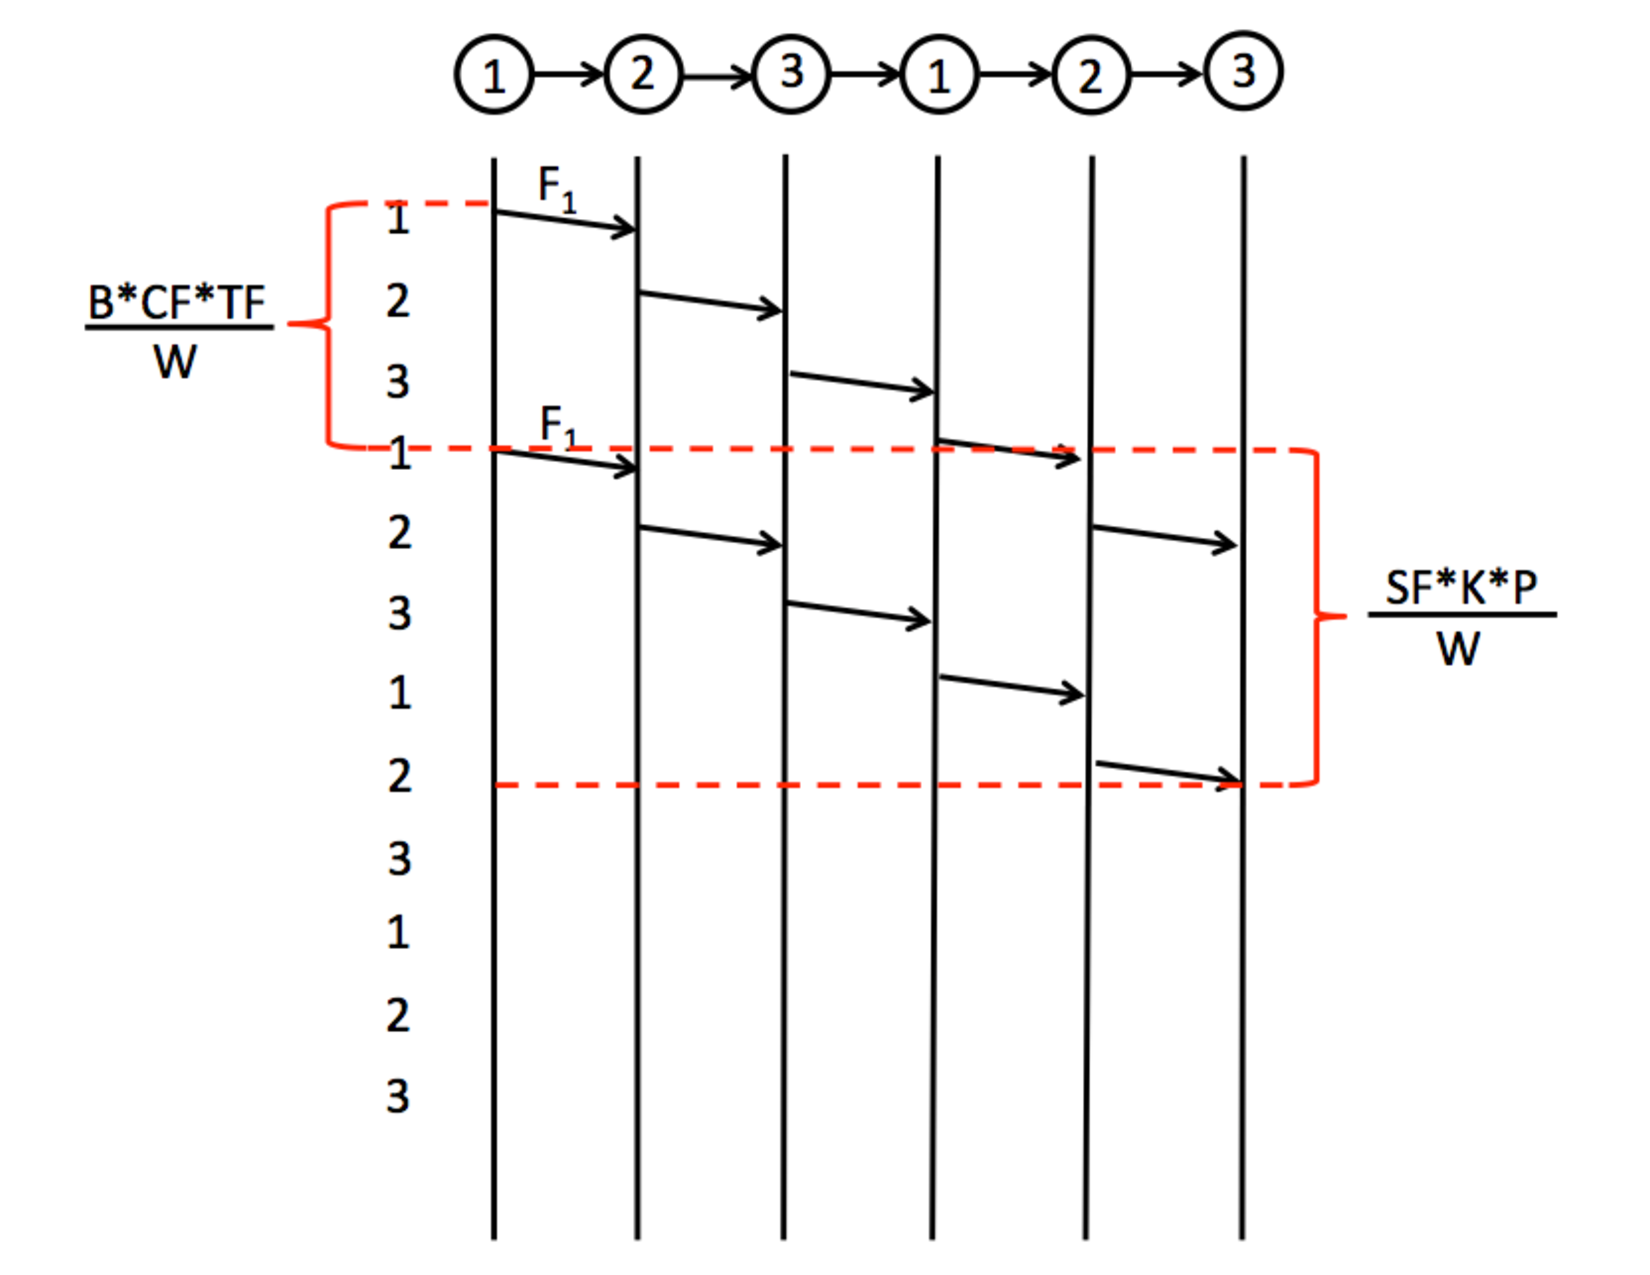
\includegraphics[scale=0.35]{figures/delay_limit_expl/delay_expl_fig_1.pdf}
    \caption{TF = 1, CF = 3, SF = 1}
    \label{fig:delay_expl_fig_1}
\end{figure}

  
\begin{figure}
    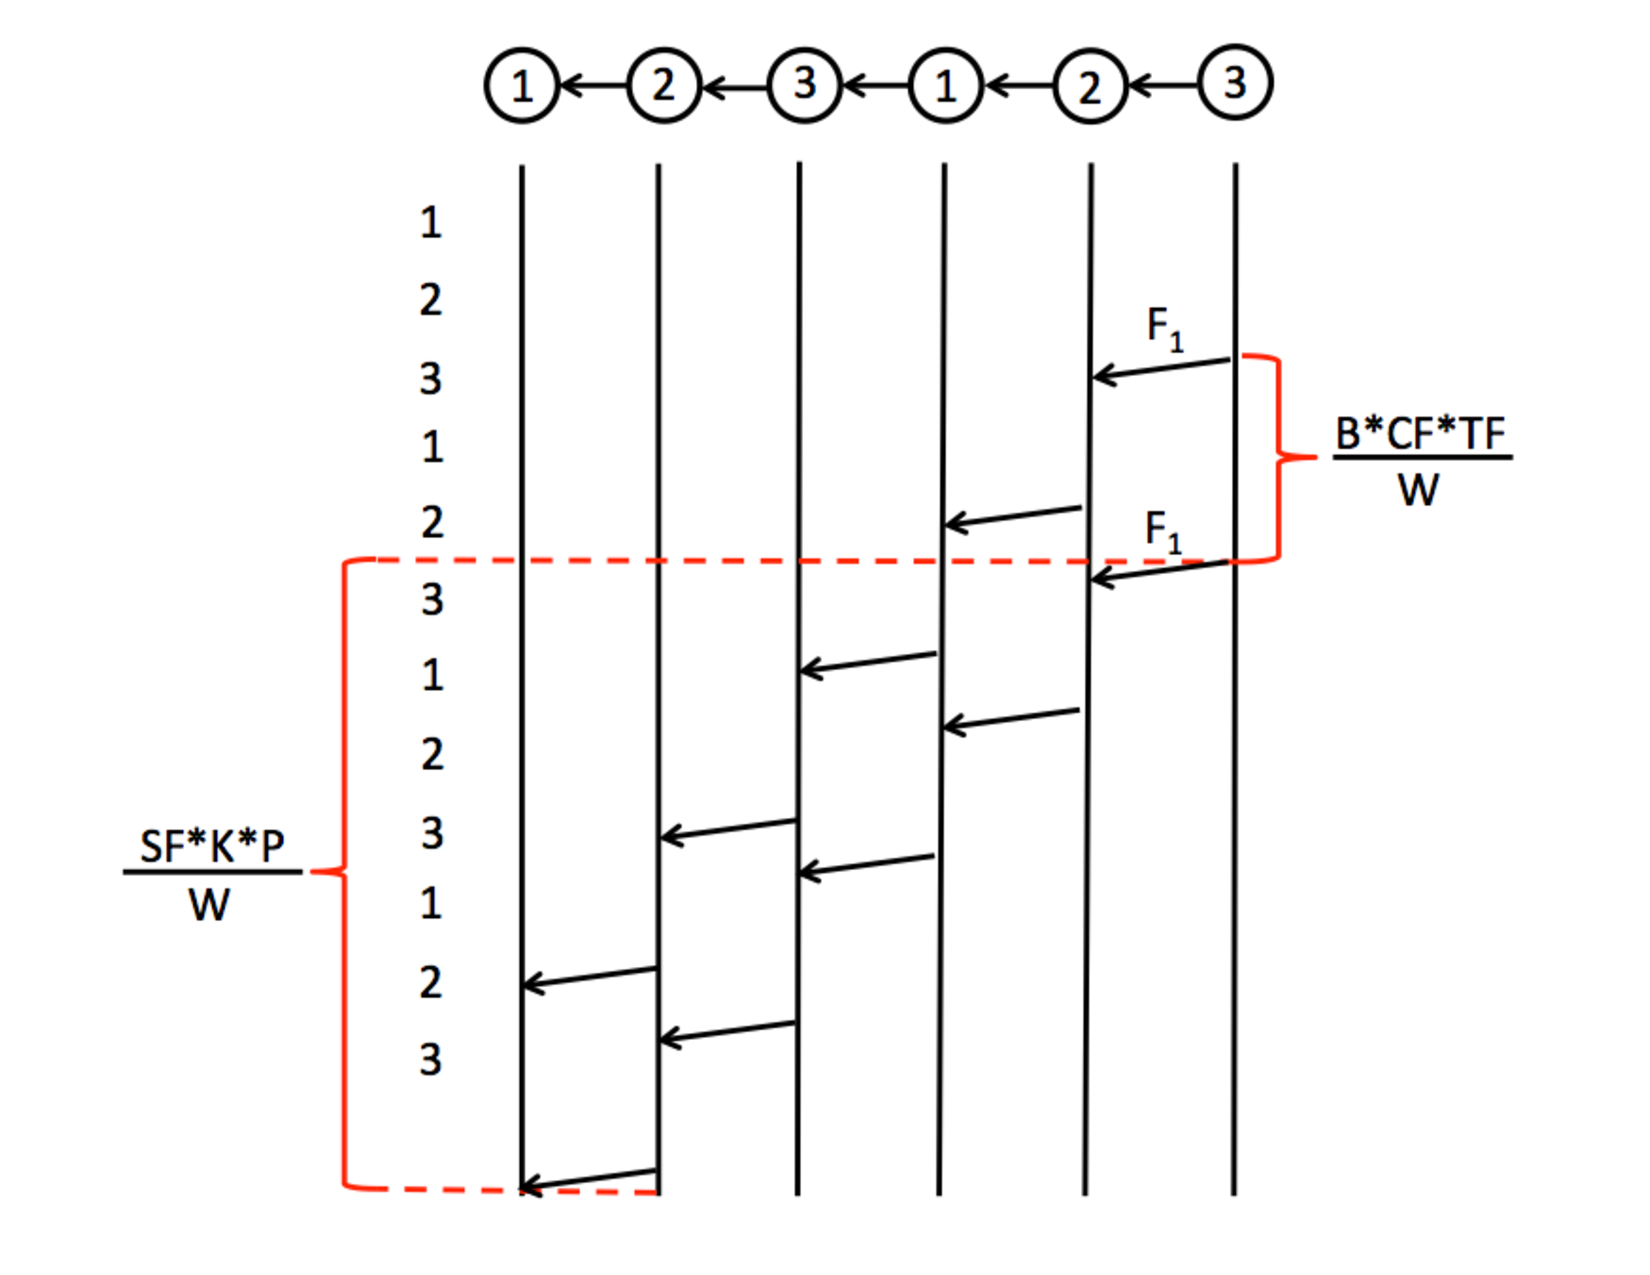
\includegraphics[scale=0.35]{figures/delay_limit_expl/delay_expl_fig_2.pdf}
    \caption{TF = 2, CF = 3, SF = 2}
    \label{fig:delay_expl_fig_2}
\end{figure}
  
\begin{figure}
    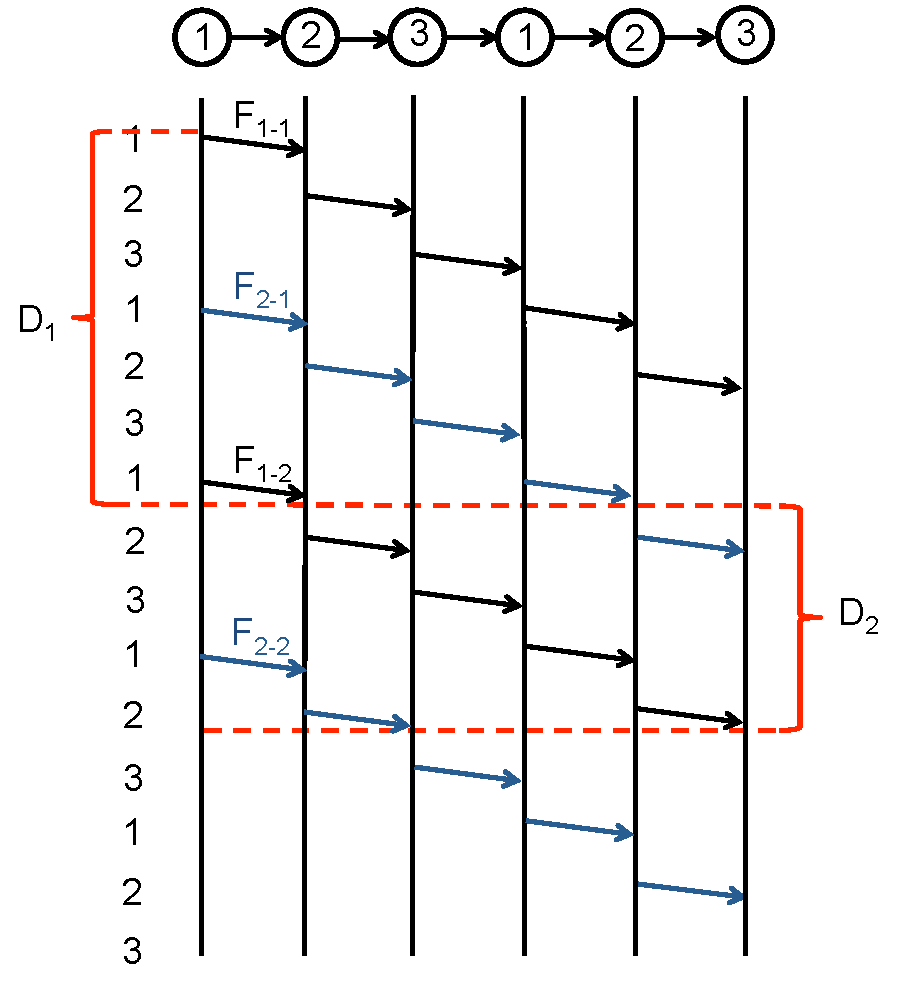
\includegraphics[scale=0.35]{figures/delay_limit_expl/delay_expl_fig_3.pdf}
    \caption{TF = 1, CF = 3, SF = 2}
    \label{fig:delay_expl_fig_3}
\end{figure}
  
\begin{figure}
    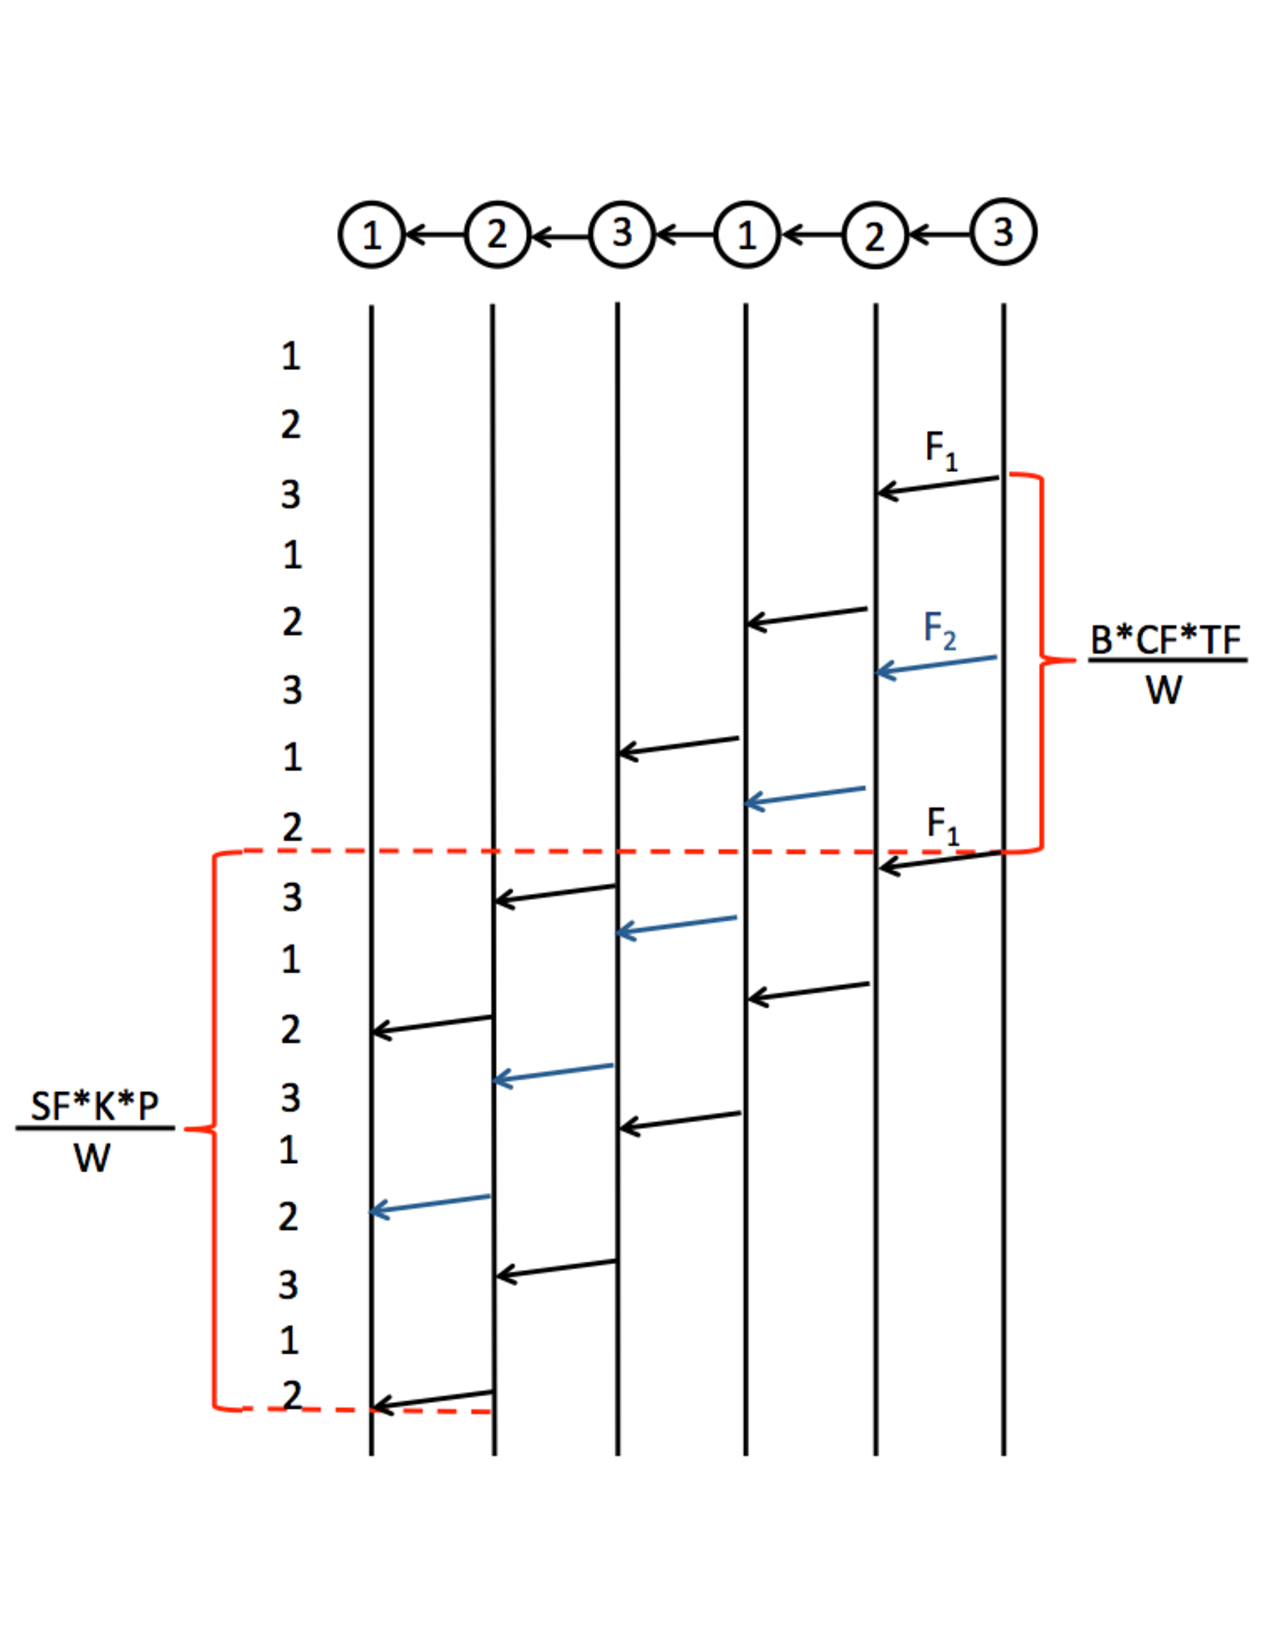
\includegraphics[scale=0.35]{figures/delay_limit_expl/delay_expl_fig_4.pdf}
    \caption{TF = 2, CF = 3, SF = 2}
    \label{fig:delay_expl_fig_4}
\end{figure}

%\appendix
%\input{sections/random_explanation}
% conference papers do not normally have an appendix


% use section* for acknowledgement
%\section*{Acknowledgment}


%The authors would like to thank...


% trigger a \newpage just before the given reference
% number - used to balance the columns on the last page
% adjust value as needed - may need to be readjusted if
% the document is modified later
%\IEEEtriggeratref{8}
% The "triggered" command can be changed if desired:
%\IEEEtriggercmd{\enlargethispage{-5in}}

% references section

% can use a bibliography generated by BibTeX as a .bbl file
% BibTeX documentation can be easily obtained at:
% http://www.ctan.org/tex-archive/biblio/bibtex/contrib/doc/
% The IEEEtran BibTeX style support page is at:
% http://www.michaelshell.org/tex/ieeetran/bibtex/
%\bibliographystyle{IEEEtran}
% argument is your BibTeX string definitions and bibliography database(s)
%\bibliography{IEEEabrv,../bib/paper}
%
% <OR> manually copy in the resultant .bbl file
% set second argument of \begin to the number of references
% (used to reserve space for the reference number labels box)
%\begin{thebibliography}{1}


\bibliographystyle{unsrt}

\bibliography{references}

%\bibitem{IEEEhowto:kopka}
%H.~Kopka and P.~W. Daly, \emph{A Guide to \LaTeX}, 3rd~ed.\hskip 1em plus
%  0.5em minus 0.4em\relax Harlow, England: Addison-Wesley, 1999.

%\end{thebibliography}




% that's all folks
\end{document}


